\documentclass[12pt]{article}

\usepackage[utf8]{inputenc}
\usepackage[backend=bibtex]{biblatex} 
\addbibresource{bibliography.bib} 
\usepackage{graphicx}


\title{Integration of KGs and PSNs for biomedical application}
\author{Lucia Mellini}
\date{}

\begin{document}

\maketitle

In the past year the literature has seen significant efforts in the automated collection, integration, and analysis of the vast amount of heterogeneous biomedical information published online. This information can be semi-automatically mined from various knowledge bases, harmonized and standardized, and condensed into integrated biomedical information structures known as knowledge graphs (KGs). In these graphs, information is represented by entities or concepts (such as proteins, drugs, and chemical compounds), which are nodes linked by edges representing known relationships.
To extract meaningful knowledge from these graphs, various graph representation learning techniques have been proposed, including random-walk based approaches and graph neural networks~\cite{Hamilton2020GraphRL}. These techniques compute representative embeddings for graph elements and use these embeddings to predict unknown categories of nodes or edges or the existence of edges between nodes.

Despite the progress in data integration research, a clear divide remains between two predictive strategies, as pointed out in the vision of ``individualized knowledge graphs''~\cite{PingPeipei2017IKGA}. On one side are predictive methods that work on datasets representing specific cases, which often yield knowledge that is not generalizable enough to be applied to compute reliable predictions on novel cases. On the other side are methods that work on KGs to uncover broad, static knowledge that is often too general for practical application. What is missing is an approach that enables predictions on specific sample data using the broad knowledge from KGs, while also deriving new relationships within a KG based on information from specific sample data. To address this issue, the first challenge is to connect these two knowledge sources. This requires an investigation into how nodes representing specific patients or samples can be linked to nodes representing broader concepts, such as genes or phenotypes. Secondly, given the vast number of nodes in a KG compared to the often limited number of cases in medical studies, new techniques should be developed to process a KG in a way that biases its representation to retain information from less represented nodes.

In our study case we consider PrimeKG~\cite{ChandakPayal2023Bakg} as our knowledge base. PrimeKG integrates 20 high-quality biomedical resources to describe 17,080 diseases with 4,050,249 relationships representing ten major biological scales. The data types integrated in the knowledge base are described by the hypergraph in Figure~\ref{fig:primekg_edge_types_hypergraph}.
\begin{figure}
    \centering
    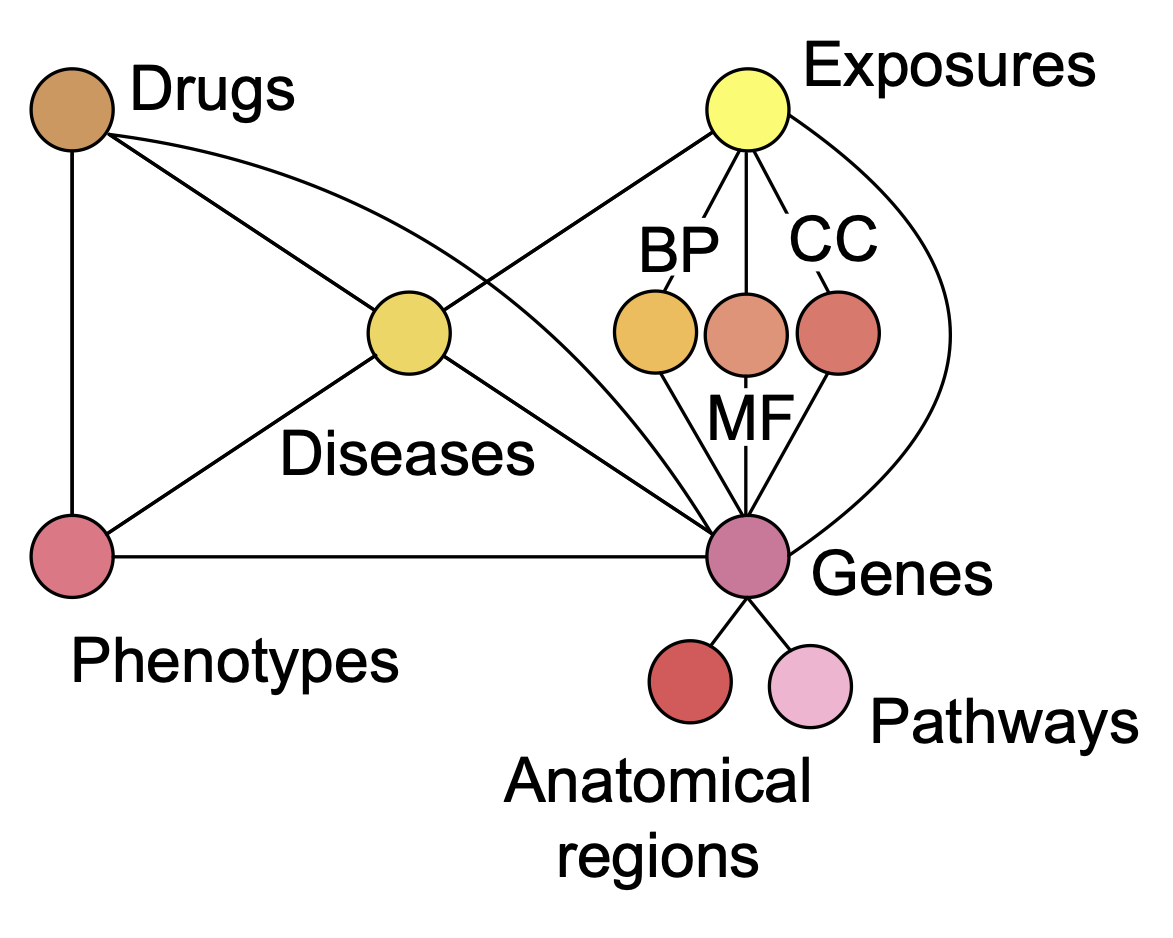
\includegraphics[width=0.6\textwidth]{figs/edge_types_hypergraph.png}
    \caption{Hypergraph of the edge types in PrimeKG}
    \label{fig:primekg_edge_types_hypergraph}
\end{figure}
In addition we use data regarding patients with Mendelian disease provided by GA4GH Phenopackets~\cite{peter_robinson_2024_13847741}. For each individual we possess their disease and their phenotypes, coupled with other features like their gender.

\printbibliography
\end{document}